%This is the third chapter of the dissertation

%The following command starts your chapter. If you want different titles used in your ToC and at the top of the page throughout the chapter, you can specify those values here. Since Columbia doesn't want extra information in the headers and footers, the "Top of Page Title" value won't actually appear.

\pagestyle{cu}
\graphicspath{{./Chapter3/Figures/}}
\chapter[The XENON1T Dark Matter Search][The XENON1T Dark Matter Search]{The XENON1T Dark Matter Search}

% https://arxiv.org/pdf/1801.07231.pdf for electron emission from wires


XENON1T is the third generation experiment of the XENON collaboration.  With a fiducial mass of $> 1000\ \mathrm{kg}$ it is the first
liquid xenon dark matter detector to reach the ton-scale era of DM detection.  Its large target mass and low radioactive background
makes it the most sensitive detector to spin-independent WIMPs.

In this chapter I describe the XENON1T experiment (\secref{sec:xenon1t_detector}) and give the results of the second science run
(\secref{sec:xenon1t_sr1}).

Lots of good info in Aprile2017b (instrument paper).

\section{The XENON1T Detector}
\label{sec:xenon1t_detector}




\subsection{PMTs}
\label{subsec:xenon1t_pmts}
A total of 248 Hamamatsu R11410-21 PMTs are installed in XENON1T.  The 127 PMTs in the top array are placed in a radial distribution to
maximize resolution of $r$ position reconstruction.  The 121 in the bottom array are packed as densely as possible to maximize light
collection.  The R11410 window is 76.2 mm in diameter and the photocathode yields an average QE to 178 nm of 34.5\% with 2.8\%
standard deviation (\citeref{Aprile2017b, Barrow2017}).  The high QE results from preselecting PMTs with $\mathrm{QE} > 28\%$ for
screening.

PMTs with the highest QE are placed in the bottom array while those with the lowest are stationed along the outside of the
top.  The difference in arrangement is strategic.  Due to liquid xenon's relatively large dielectric constant (1.95) an S1 will
often reflect off the surface and be redirected towards the bottom of the TPC.  For low-energy events - the relevant range for WIMP DM
searches - a nuclear recoils may only emit a small number ($\lesssim 100$) of photons, many of which never reach the PMTs.  Thus it is
most advantageous to position those with the highest quantum efficiency in the region most likely to see scintillation from an
S1.  Likewise, S2s easily produce enough scintillation to be observed by both arrays.  Therefore the QE of the top PMTs is comparatively
unimportant, and may even be advantageous for larger S2s where saturation can occur.  The layout of the PMTs with respect to QE is shown
in \figref{fig:xenon1t_pmt_qe}.

\begin{figure}
\centering
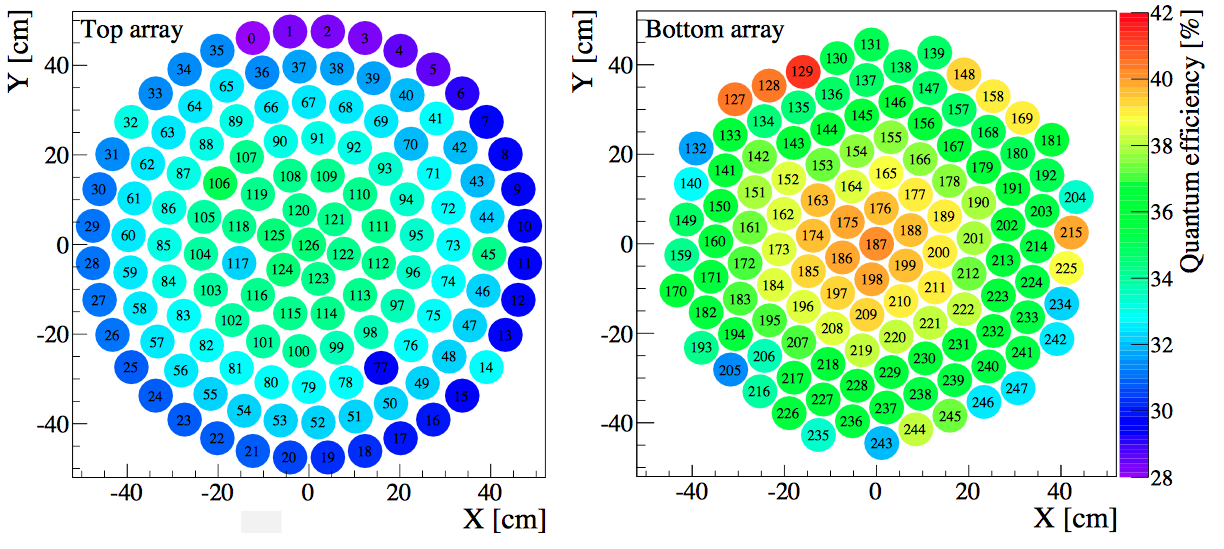
\includegraphics[width=\textwidth]{PMTQuantumEfficiency}
\caption{Quantum efficiency of top (left) and bottom (right) PMT arrays.  PMTs with highest QE are placed in the center of the bottom
array to maximize light collection while those with the lowest are placed in the outer region of the top.  Image credit:
\citeref{Aprile2017b}.}
\label{fig:xenon1t_pmt_qe}
\end{figure}

\begin{figure}
    \centering
    \begin{subfigure}[t]{0.45\textwidth}
        \centering
        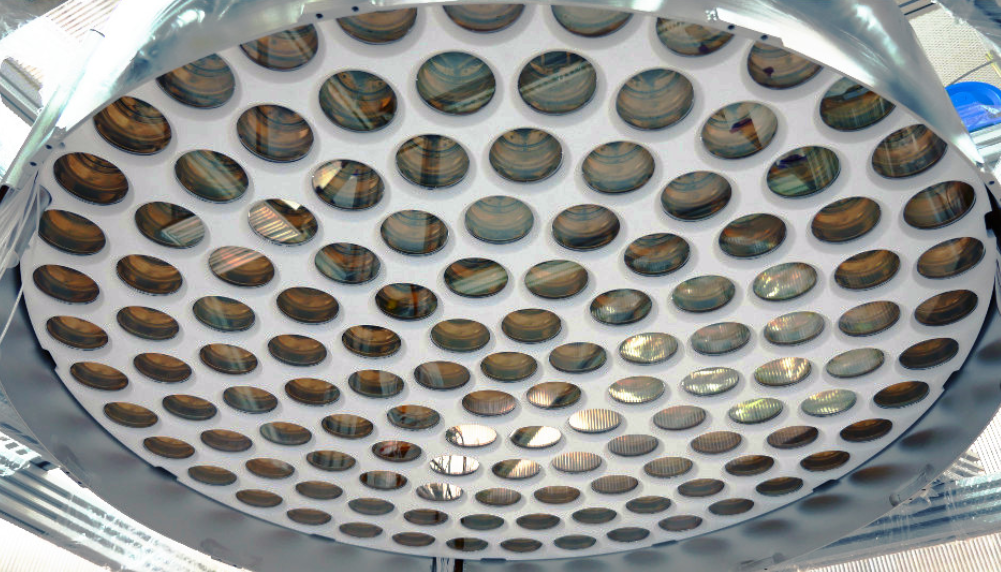
\includegraphics[height=4.5cm]{PMTTopArray}
    \end{subfigure}%
    \begin{subfigure}[t]{0.45\textwidth}
        \centering
        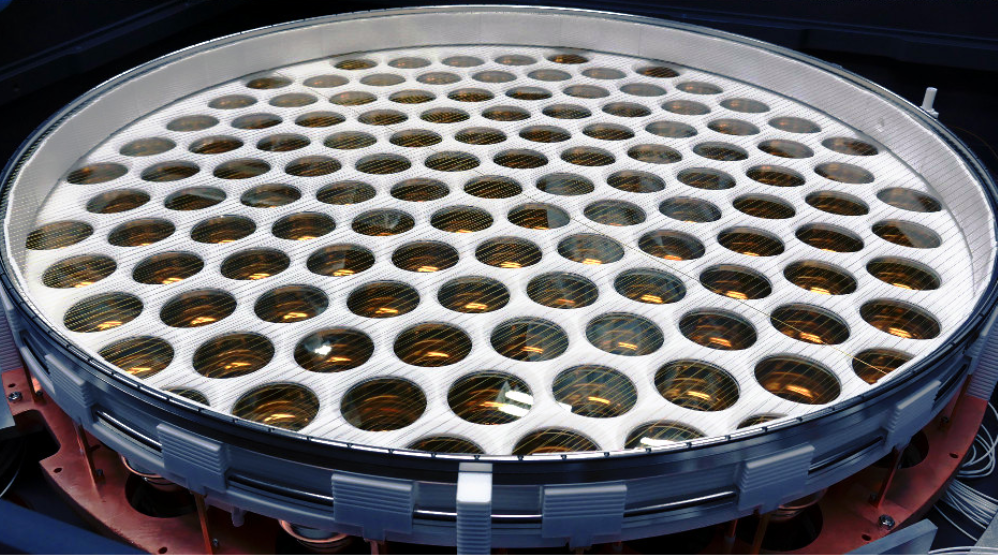
\includegraphics[height=4.5cm]{PMTBottomArray}
    \end{subfigure}
    \caption{XENON1T top (left) and bottom (right) PMT arrays.  Top PMTs are installed inside the diving bell in a radial distribution
    to minimize uncertainty in radial position reconstruction.  Bottom PMTs are installed below the cathode and screening mesh that
    limits interference between the PMT and cathode electric fields, both of which can be seen in the figure.  They are packed tightly
    together to maximize lightcollection.  Image credit: \citeref{Aprile2017b}.}
	\label{fig:xenon1t_pmt_array}
\end{figure}

\begin{figure}
\centering
\includegraphics[width=0.8\textwidth]{Fig1FromAprile2015}
\label{fig:xenon1t_hamamatsu_pmt}
\end{figure}

The R11410-21 has 12 dynodes following the focusing electrode disk.  The first dynode is the largest and extends to the electrode to
maximize the probability of capturing photoelectrons.  A schematic can be be seen in \figref{fig:xenon1t_hamamatsu_pmt}.  The electrode,
dynode, and shield are stainless steel and are insulated with L-shaped quartz plates.  The window is
also made of quartz, since it is transparent to vacuum ultraviolet (VUV) photons.  Deposited on it is a low-temperature bialkali
photocathode.  The window is fixed with an aluminum seal to the faceplate flange, which along with the stem flange is constructed from
Kovar.  Because of the PMT body's large mass (71\% of total Kovar, 35\% of total) a low-\ce{^{60}Co} Kovar is chosen.  Finally, to insulate
the connections to each dynode the stem is ceramic.

Because radioactivity limits the fiducial volume and increases the event rate, making accidental coincidence and outlier events more
likely, XENON and Hamamatsu worked together to develop a highly radio-pure PMT.  There were several iterations of the R11410 model before
the R11410-21 was determined to be adequate.  Nearly all the \ce{^{137}Cs} and \ce{^{60}Co} comes from the Kovar, though the \ce{^{137}Cs}
content is negligible and the \ce{^{60}Co} is 3-10 times lower than older models.  The remaining screened isotopes, \ce{^{238}U},
\ce{^{228}Th}, \ce{^{228}Ra}, \ce{^{226}Ra}, and \ce{^{40}K}, are dominated by the ceramic stem (\citeref{Aprile2015}).  Unfortunately a
material that is more radio-pure and can insulate the dynode connections has not been found.  Sapphire was used in an iteration but
ultimately showed any improvement was minimal.

The dark count rate, or the number of signals per second above a threshold without a light source, is an important property to
characterize.  At ambient temperatures the primary cause is thermal electrons that scale with PMT voltage.  This becomes subdominant at
cryogenic temperatures to electron field emission and radioactivity (internal and external) as well as cosmic rays.  In a detector such
as XENON1T higher dark count rates make accidental coincidence more likely, which produces fake additional background and in the worst case
can place fake events in the signal region.  Because the rate is dependent on the threshold it can effectively be tuned.  However, because
for DM search we would like as low of a threshold as possible, choosing PMTs with low dark count rate is essential.

Another problematic feature is light emission from the phototube itself, where light is created inside the PMT and escapes through the
window.  It has been observed to mainly occur in one of two ways.  The first is through a discharge of intense light that can last for
several seconds.  This so-called ``flash" is bright enough to be easily observable to itself and by PMTs that are facing its
window.  However, the intensity can be so strong that it can take anywhere from several minutes to several hours for them to
recover.  Because they seem to occur spontaneously and are not well understood it is impossible to predict when a flash will occur.

The second variety is a subtle but often continuous stream of light.  Known as ``micro light emission" it is considerably harder to
identify.  Doing so requires facing two phototubes towards one another and measuring the dark rate of each one with and without the other
on.  The level of emission increases with temperature and bias voltage.  Keeping the PMTs at cryogenic temperatures during DM runs reduces
such effects, and voltages can be lowered to help further.  Still, if micro light emission continues the PMT cannot be used as it risks
contaminating the detected light from the true event population.

Directly following the pulse of a PMT hit a secondary pulse may occur.  Known as afterpulses, they can occur within 10s of
nanoseconds.  This can make them difficult to resolve from true pulses - especially S2s - that can have widths of several
microseconds.  However, they are an inevitable side effect when using PMTs so characterizing them properly is important.  There are three
mechanisms known to cause afterpulses.

The first is elastic scattering of the photoelectron with the first dynode, freeing \electron that shortly return to the dynode.  This
prompts afterpulses in the range of a few to tens of nanoseconds.  A second kind is thought to stem
from dark noise and single electrons but is not well understood.  It has a relatively uniform distribution in delay time up to several
microseconds.  Both of these afterpulses have relatively small areas of $\lessim 2\ \mathrm{PE}$.

A photoelectron may occasionally ionize residual gas inside the PMT along its trajectory to the first dynode.  The molecule then drifts
towards the photocathode, expelling additional electrons.  The number of newly ejected electrons (area of afterpulse) depends
on the ion and the position of ionization.  The responsible ion can be determined by calculating the time between the true pulse and
afterpulse.  For R11410-21 this gives

\begin{equation}
\delta t_{\mathrm{ap}} = \frac{\pi}{4} \sqrt{\frac{2 m}{q V_{0}}} L
\end{equation}

where $\delta t_{\mathrm{ap}}$ is the delay time, $m$ and $q$ are the ion's mass and charge, and $V_{0}$ and $L$ are the potential
difference and length between the photocathode and first dynode (see \citeref{Barrow2017} for details).  Note that $\delta t_{\mathrm{ap}}$
does not depend on where the ionization occurred.  Thus, if we know the time between the true and afterpulse the ion - or more specifically
charge to mass ratio - can be calculated.  Pulse time differences range from several hundred nanoseconds to several microseconds.  These
correspond to the ``lines" in \figref{fig:xenon1t_pmts_ap} that extend to larger afterpulses.  The short timescales of S1s make them
unlikely to be grouped with an afterpulse, though for S2s this is more likely.

\begin{figure}
\centering
\includegraphics[width=\textwidth]{Afterpulse}
\caption{Afterpulses for one of the PMTs from XENON1T.}
\label{fig:xenon1t_pmts_ap}
\end{figure}

Because it is not possible to remove all residual gas any PMT will suffer from some ionization-based afterpulsing.  A better vacuum
corresponds to fewer afterpulses and a healthier PMT in general.  If the concentration of gas in the PMT vacuum were to increase it would
escalate the afterpulse rate.  Therefore if when using in xenon the Xe peaks grow over time the PMT most likely has a leak and should
be removed, as continued worsening of the vacuum will lead to deterioration and inability to operate the PMT.  All PMTs were tested before
being installed in XENON1T.  73 were rejected and replaced: 12 due to high dark count rates, 53 for light emission, and 8 for
afterpulsing.

An additional six Hamamatsu R8520 PMTs reside in LXe outside the TPC near the top electrode for studying calibrations.  These PMTs have
been used in a number of LXe TPCs including XENON100, the predecessor to XENON1T (\citeref{Goetzke2017}, see \citeref{Aprile2012} for
details on XENON100).

\begin{figure}
\centering
\includegraphics[width=0.8\textwidth]{Fig4Barrow2017}
\caption{(Left) Single photoelectron spectrum.}
\label{fig:xenon1t_pmt_spe}
\end{figure}




\subsection{TPC}
\label{subsec:xenon1t_tpc}

\begin{figure}
\centering
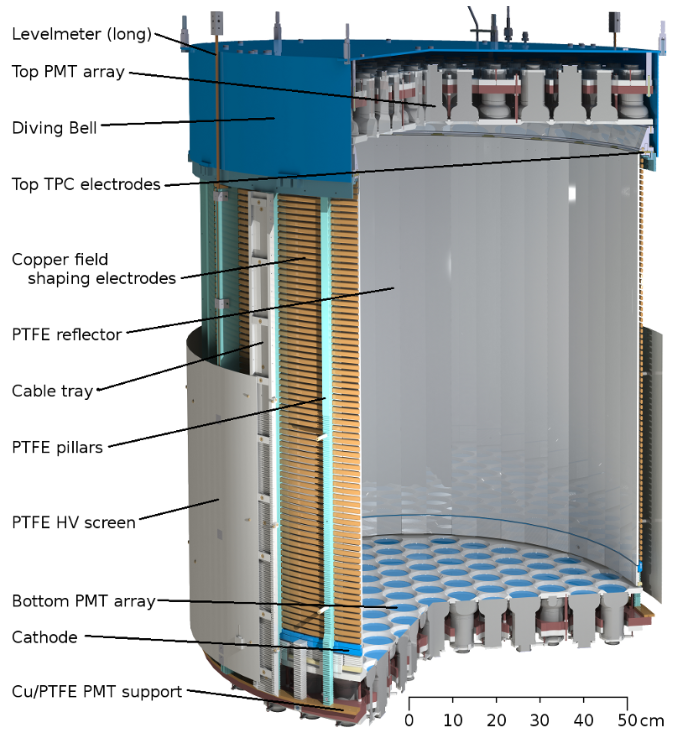
\includegraphics[width=0.8\textwidth]{XENON1TTPC}
\label{fig:xenon1t_tpc_tpc}
\end{figure}

\begin{figure}
\centering
\incluegraphics[width=0.6\textwidth]{Fig3Aprile2017b}
\label{fig:xenon1t_tpc_efield}
\end{figure}



\begin{figure}
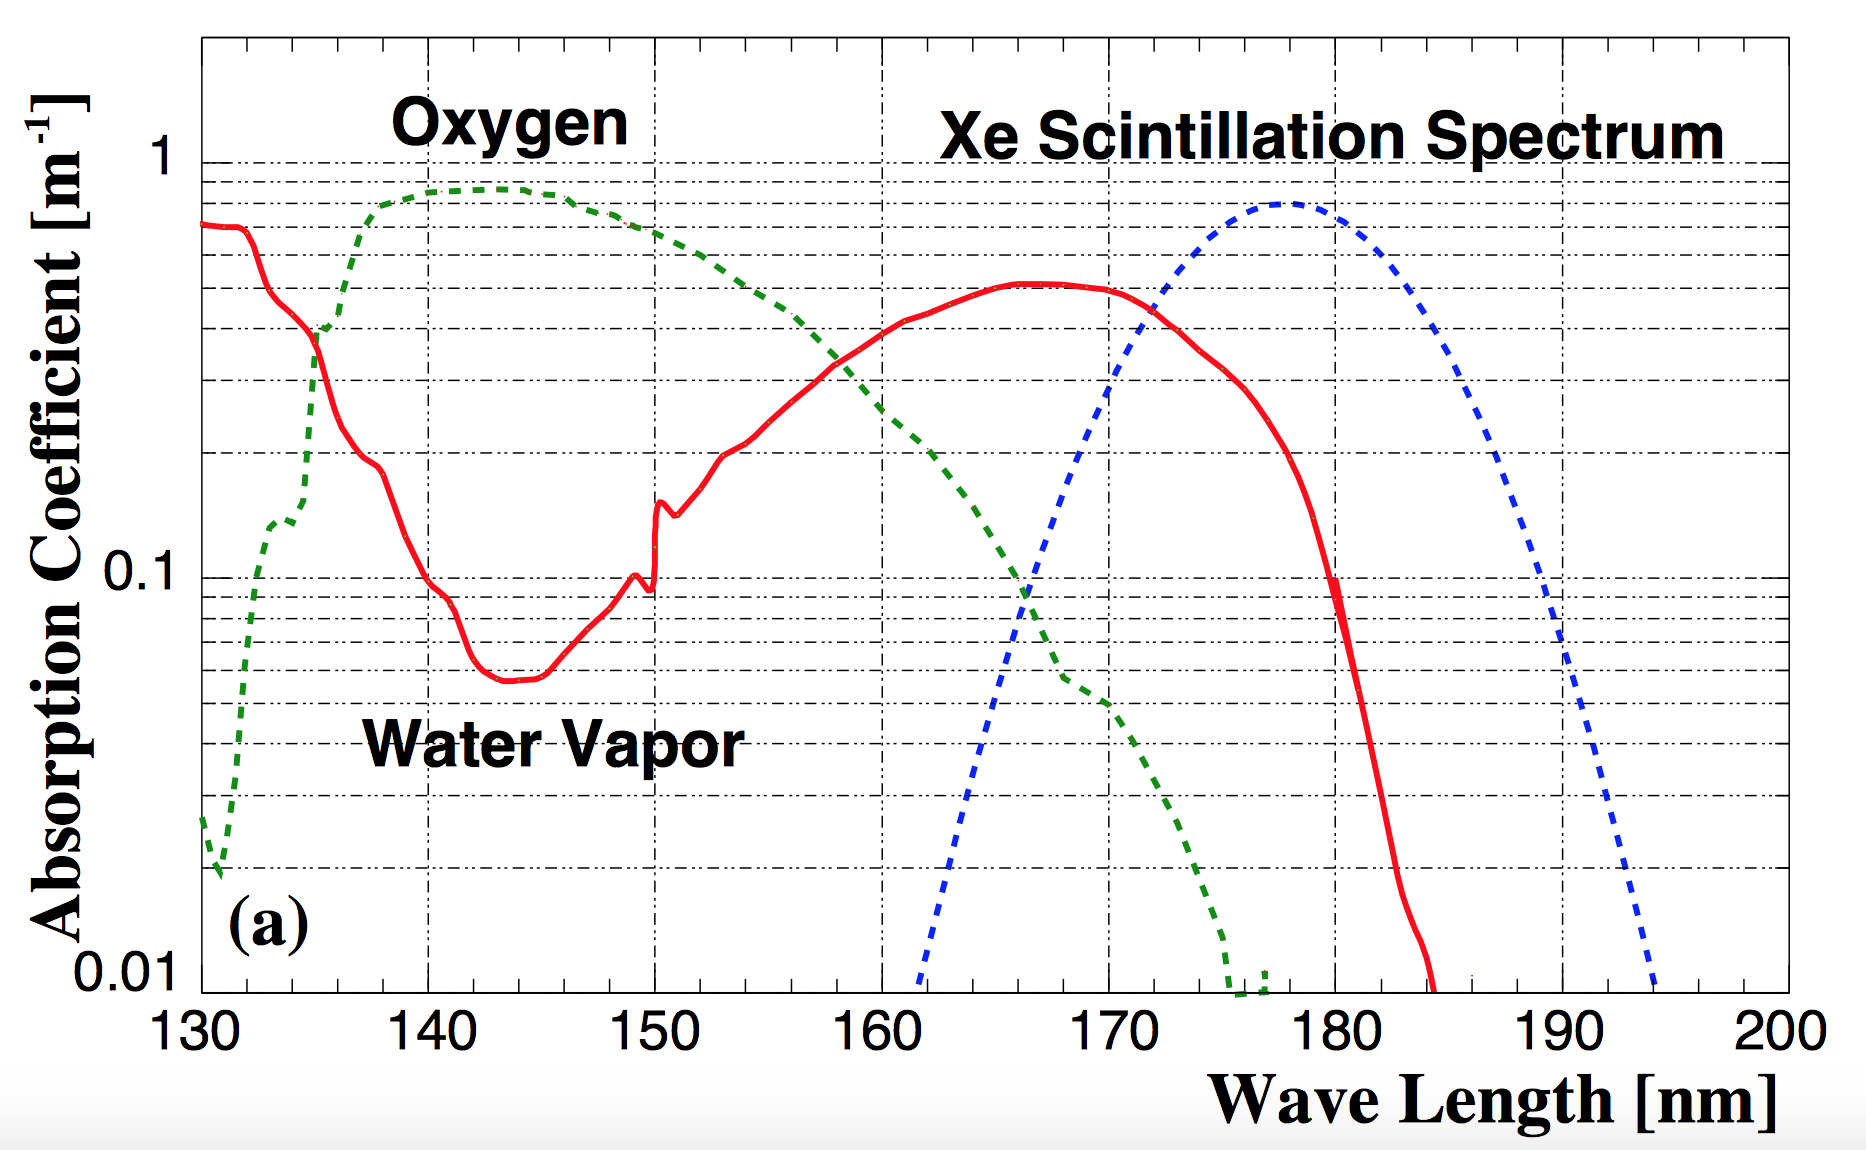
\includegraphics[\width=0.8\textwidth]{AbsorptionSpectra}
\caption{\citeref{Ozone2005}}
\end{figure}


In an electric field $E$ an \electron that is freed but does not recombine with its parent or other ionized atoms will move anti-parallel
to the field at drift velocity $v_{d}$.  For $E \lesssim 100\ \mathrm{V\ cm^{-1}}$ \vd$\propto E$, $100 \lesssim E \lesssim 10^{3-4}$
\vd$\propto E^{1/2}$, and $E \gtrsim 10^{4}$ \vd plateaus at $\sim 3\ \mathrm{mm\ \mu s^{-1}}$ (\citeref{Miller1968}).

\begin{table}
 \centering
 \begin{tabular}{cc}
 \hline
 $E$ [V cm$^{-1}$] & \vd [mm $\mu$s$^{-1}$] \\
 \hline
 $\lesssim 100$ & \vd$\propto E$ \\
 $\sim 100-10^{3-4}$ & \vd$\propto E^{1/2}$ \\
 $\gtrsim 10^{4}$ & \vd$\sim 3$ \\
 \hline
 \caption{Drift velocity \vd as a function of electric field $E$ for LXe}
 \end{tabular}
\end{table}

\begin{figure}
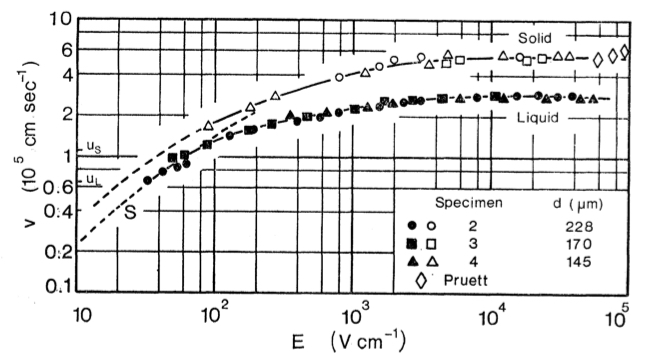
\includegraphics[angle=0.5, width=0.8\textwidth]{DriftVelocity}
\caption{Drift velocity for solid and liquid xenon}
\label{fig:drift_velocity}
\end{figure}

As the electron cloud drifts it will diffuse both longitudinally (in the direction of $E$) and transversely (perpendicular to $E$).  The
diffusion coefficients $D_{L}$ and $D_{T}$ are dependent on the electric field with $D_{T}/D_{L} \sim 10$.  The electron spread can
be written as $\sigma_{D_{T}} = \sqrt{D_{T} t_{d}}$ where $t_{d} = d/v_{d}$ is the drift time and $d$ is the drift distance.

Extensive xenon distillation and purification occurs before it is used in a detector.  Nonetheless impurities outgas from detector
material and contaminate the LXe.  Electronegative impurities in particular present a problem since they will attach to a free \electron,
lowering the number that reach the top of the detector and decreasing the secondary scintillation as shown in \eqref{eq:impurity_attach}.

\begin{equation}
e^{-} + S \rightarrow S^{-}
\label{eq:impurity_attach}
\end{equation}

\noindent The amount of \electron captured is dependent on the time in the LXe.  Thus an advantage of larger \efields is a larger
\vd (up to a point) and thus less time in the liquid.  Doping LXe with organic materials such as butane can increase \vd at higher
\efields but they are not used in DM detectors due to difficulty in purifying (\citeref{Yoshino1976}).  By setting the rate at which
electrons are absorbed by impurities $dq/dt = -qk_{S}S$ where $S$ is the impurity concentration and $k_{S}$ is the attachment rate
constant we find

\begin{equation}
q(t) = q_{0}e^{-tk_{S}S} = q_{0}e^{-t/\tau_{e}}
\label{eq:lifetime_equation}
\end{equation}

\noindent where $\tau_{e} = (k_{S}S)^{-1}$ and is known as the electron lifetime.  $k_{S}$ is shown in \figref{fig:attachment_rate} for
O$_{2}$,
N$_{2}$O, and SF$_{6}$.  We see that for N$_{2}$O the attaching rate constant increases with \efield whereas \otwo and SF$_{6}$
decerase.  Typically impurity concentration is given in O$_{2}$-equivalent values - that is, the concentration of \otwo if it was solely
responsible for \electron attachment.  For modeling electron lifetime it turns out that using the \otwo curve in
\figref{fig:attachment_rate} gives a good approximation.  Removing such impurities will be discussed in detail in \secref{}.

\begin{figure}
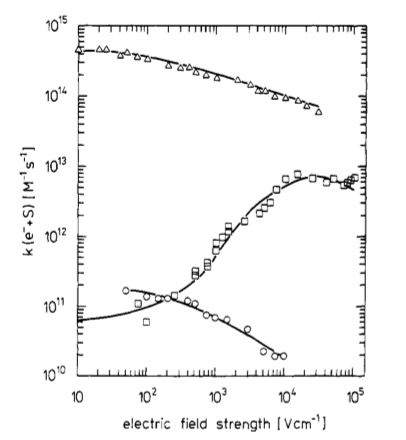
\includegraphics[width=0.8\textwidth]{AttachmentRate}
\caption{Attaching rate constant $k_{S}$ from \citeref{Bakale1976} for \otwo, N$_{2}$O, and SF$_{6}$ with respect to electric field.  At
larger \efield $k_{S}$ increases for N$_{2}$O and decreases for \otwo and SF$_{6}$.}
\label{fig:attachment_rate}
\end{figure}

In a TPC a cathode at the bottom of the detector applies an electric field in the LXe.  The \electron drift towards the top where a
grounded gate rests a few millimeters below the LXe surface.  Directly above the gate by a couple centimeters is the anode, which
applies a strong electric field that extracts the electrons into the gas xenon (GXe).  An extracted electron will ionize and excite
GXe atoms, whose freed electrons will do so as well in what is known as electroluminescence.  The number of ionized and excited atoms
is proportional to the number of \electron extracted, hence it is also known as proportional scintillation.  The number of photons
$N_{\mathrm{ph}}$ produced traveling a distance $z$ is

\begin{equation}
\frac{dN_{\mathrm{ph}}}{dz} = \alpha \Big( \frac{E_{g}}{P} - \beta \Big) P
\label{eq:electronlum}
\end{equation}

\noindent where $\alpha = 70\ \mathrm{photons\ kV^{-1}}$, $\beta = 1.0\ \mathrm{kV\ cm^{-1}\ atm^{-1}}$, and $E_{g}$ and $P$ are the
GXe electric field and pressure, respectively (\citeref{Belogurov1995}).

For PMT use Fig. 1 of Aprile2015